\documentclass[11pt]{report}
\usepackage{geometry}                % See geometry.pdf to learn the layout options. There are lots.
\geometry{a4paper}                   % ... or a4paper or a5paper or ... 
\usepackage{listings}
%\usepackage[parfill]{parskip}    % Activate to begin paragraphs with an empty line rather than an indent
\usepackage{graphicx}
\usepackage{amssymb}
\usepackage{epstopdf}
\usepackage[usenames, dvipsnames, table]{xcolor}
\usepackage{hyperref}
\usepackage[utf8]{inputenc}
\usepackage{multicol}

\DeclareGraphicsRule{.tif}{png}{.png}{`convert #1 `dirname #1`/`basename #1 .tif`.png}

\newcommand{\leongage}{NoBeard}

\newcommand{\alternative}{$\mid \;$}
\newcommand{\emptystring}{$\varepsilon$}

% ---------------------------------------------- Definition of grammar environment -----------------------------------------------------
\newenvironment{grammar}[2] % two arguments: width of left side and width of right side of grammar
	{
		\newcommand{\completerule}[2]{##1 & = & ##2.\\}
		\newcommand{\startrule}[2]{##1 & = & ##2\\}
		\newcommand{\alternativerule}[1]{ & $|$ & ##1\\}
		\newcommand{\alternativeend}[1]{ & $|$ & ##1.\\}
		\newcommand{\finishrule}[1]{ & & ##1.\\}
		\begin{tabular}{p{#1} c p{#2}}
	}
	{	\end{tabular}
	}

% ----------------------------------------------- Definition of attributed grammar environment
\newenvironment{atg}[1][6cm]
	{\begin{tabular}[b]{lclp{#1}}}
	{\end{tabular}}
\newcommand{\atgsy}[2]{$\textrm{#1}_\textrm{#2}$}
\newcommand{\outattr}{$\uparrow$}
\newcommand{\inattr}{$\downarrow$}

\newcommand{\semantics}[1]{\textcolor{Gray}{#1}}

\newenvironment {sem}
	{\underline{sem}}
	{\underline{endsem}}
	
\newcommand{\where}{\underline{where} }

% --------------------------------------------------- Definition of colors used in source code listings ----------------------------------------------
\definecolor{srcred}{rgb}{0.6,0,0}
\definecolor{srcpurple}{rgb}{0.5,0,0.35}
\definecolor{srcgreen}{rgb}{0.25,0.5,0.35}
\definecolor{srcblue}{rgb}{0.25,0.35,0.75}

% -------------------------------------------------- Definition of lstlisting for NoBeard ------------------------------------------------------------------
\lstdefinelanguage{NoBeard}{
	basicstyle=\ttfamily,
	frame=single,
	sensitive=true,
	morekeywords = {unit, function, do, done, int, char, put, putln},
	morecomment=[l][\color{srcgreen}]{\#},
	morestring=[b][\color{srcred}]{"},
	keywordstyle=\color{srcpurple},
	showspaces=false,
	showstringspaces=false
}

% ----------------------------------------------- Definition of lstlisting for NoBeardAsm programs --------------------------------------------------
\lstdefinelanguage{NoBeardAsm}{
	basicstyle=\ttfamily,
	frame=single,
	sensitive=true,
	tabsize=3,
	morekeywords = {nop, lit, la, lv, lc, sto, stc, assn, neg, add, sub, mul, div, mod, not, rel, fjmp, tjmp, jmp, in, out, inc, halt},
	morecomment=[l][\color{srcgreen}]{\#},
	morestring=[b][\color{srcred}]{"},
	keywordstyle=\color{srcpurple},
	showspaces=false,
	showstringspaces=false,
	escapechar=|,
	captionpos=b,
	numberstyle=\small
}

% --------------------------------- Definition of lstlisting for AsmDef the language to define assembler commands -----------------------
\lstdefinelanguage{AsmDef}{
	basicstyle=\ttfamily,
	frame=single,
	sensitive=true,
	tabsize=3,
	morekeywords = {push, pop, printf, dat, prog, top, fp, pc, ms},
	morecomment=[l][\color{srcgreen}]{//},
	morestring=[b][\color{srcred}]{"},
	keywordstyle=\color{srcpurple},
	showspaces=false,
	showstringspaces=false
}

% ------------------------------------------------------ Definition of assembler instruction commands --------------------------------------------
\newcommand{\onebyteinstruction}[1]{
\begin{tabular}{|p{3.9em}|}
\hline
\tiny{Byte 0} \\ \hline
#1  \\ \hline
\end{tabular}
}

\newcommand{\twobyteinstruction}[2]{
\begin{tabular}{|p{3.9em}|p{9em}|p{9em}|}
\hline
\tiny{Byte 0} & \tiny{Byte 1} \\ \hline
#1 & #2 \\ \hline
\end{tabular}
}

\newcommand{\threebyteinstruction}[2]{
\begin{tabular}{|p{3.9em}|p{9em}|p{9em}|}
\hline
\tiny{Byte 0} & \tiny{Byte 1} & \tiny{Byte 2} \\ \hline
#1 & \multicolumn{2}{c |}{#2} \\ \hline
\end{tabular}
}

\newcommand{\fourbyteinstructiona}[3]{
\begin{tabular}{|p{3.9em}|p{9em}|p{9em}|p{9em}|}
\hline
\tiny{Byte 0} & \tiny{Byte 1} & \tiny{Byte 2} & \tiny{Byte 3} \\ \hline
#1 & #2 & \multicolumn{2}{c |}{#3} \\ \hline
\end{tabular}
}


% ---------------------------------------------------------------------- Start of document -----------------------------------------------------------------
\begin{document}
\begin{titlepage}
\begin{center}

\includegraphics[scale=0.3]{no_beard_1.jpg} \\[2em]
{\Huge A Formal Description of \leongage} \\[1em]
{\large v 1.2} \\[2em]
{\Large P. Bauer} \\[1em]
HTBLA Leonding \\
Limesstr. 14 - 18 \\
4060 Leonding \\
Austria
\end{center}
\end{titlepage}

\section*{Revisions}
\begin{tabular}{|l|l|p{.5\textwidth}|}
\hline
\cellcolor{Gray}\textcolor{White}{Date} & \cellcolor{Gray}\textcolor{White}{Author} & \cellcolor{Gray}\textcolor{White}{Change} \\ \hline
September 21, 2016 & P. Bauer & Added instructins in.  \\ \hline
September 2, 2016 & P. Bauer & Added instructins lci, lvi.  \\ \hline
August 15, 2016 & P. Bauer & Added introduction to assembler.  \\ \hline
August 9, 2016 & P. Bauer & Explained call stack and control unit of the machine.  \\ \hline
June 25, 2016 & P. Bauer & Added more detailed description of the machine and added all assembler instructions used so far.  \\ \hline
June 12, 2016 & P. Bauer & Changed environment for grammar and formatting of source code. \\ \hline
June 5, 2014 & P. Bauer & {\bf Released v. 1.1}  \\ \hline
June 5, 2012 & P. Bauer & {\bf Released v. 1.0}  \\ \hline
\end{tabular}

\pagebreak

\tableofcontents
\chapter{Introduction}
\section{The \leongage{} Project}
This project aims to provide students who want to dig into the fields of assembler programming, system programming and compiler construction a playground where they can experiment in a pretty small and clean environment. The components developed here do not have the quirks and compromises real machines, assemblers, and compilers have to make in order to keep up with their real life requirements. In particular the following parts are provided:

\begin{itemize}
	\item The {\em \leongage{} Machine}. A virtual machine with an instruction set of less than 30 instructions which is pretty easy to grasp compared to the instruction set sizes of real life machines. The machine is purely stack based such that the structure of each instruction is again easy to understand and to follow.
	\item The {\em \leongage{} Assembler}. To write programs for the \leongage{} Machine an assembler is provided. In the published version of the project no support of labels, symbolic variables, etc. is given. Here the focus is to direct the students to the very basics of how machine programs for the \leongage{} Machine look like and how they work. Extensions as the ones mentioned above can be done by the interested student as an exercise.
	\item The {\em \leongage{} Compiler}. To facilitate programming for the \leongage{} Machine and to give insights into the basic techniques of compiler construction a dedicated language is defined and the corresponding compiler is implemented. We did not go for the automated construction of compilers with compiler generators since we wanted to emphasize the direct relationship of formal grammars to parsers using the recursive descending method. For students interested in compiler construction using compiler generators the great book of Pat Terry~\cite{terry_compiling_2004} is recommended.
\end{itemize}

\section{Trivia and Acknowledgements}
The \leongage{} tools are used to support the courses {\em Technical Informatics} and {\em Programming and Software Engineering} (in particular the part {\em Theoretical Informatics}) held for third grade students of the Department of Informatics at the HTBLA Leonding. Therefore the students of these grades are forced to go through this material in more detail. All remarks from students of the former years helped to improve the project and to bring it into the shape as it is today. A big Thank You at this point is the least one can do in return for that. Since the whole project is still ongoing: In case of typos, misleading wording or other problems, please feel free to contact the author. Any help in this direction is highly appreciated.

According to a web article (see \cite{khason_computer_2008}) the popularity of programming languages is strongly related to the fact whether its inventor(s) is a / are  bearded m[ae]n or not. Well, the main aim of the programming language \leongage{} is not to be popular,
moreover it should give the reader a clear insight how the main principles of assembler programming, system programming, and compiler construction are. This is the background of the name of the whole project. Thanks to my former colleagues Peter Penz, Hugo Koblmüller, and Harald Wick for their constant friendship and creativity which not only helped me to find a proper name for this project.

When developing this project we had an extremely helpful guideline in the {\em MiniModula2} project developed by Hanspeter Mössenböck at the Johannes Kepler University in Linz~\cite{mossenbock_formale_1991}. Actually all basic concepts used here are stolen from this project.

\section{Structure}


\chapter{The \leongage{} Machine}
\lstset{language=AsmDef}
\section{Overview}
The virtual machine being target for \leongage{} programs is a stack machine with instructions of variable length and has the following components. The word width of the \leongage{} machine is four bytes.

\subsection{Program Memory}
The program memory is further denoted as \lstinline$prog[MAX_PROG]$. It is byte addressed with a maximum size of \lstinline$MAX_PROG$. Attempts to access addresses outside the range of 0 to \lstinline$MAX_PROG - 1$ result in a \lstinline$ProgramAddressError$.

\subsection{Data Memory}
The {\em data memory} is byte addressed and storage is done in the following way:

\begin{itemize}
\item Characters are one-byte values and are stored byte-wise into the data memory.
\item Integers are four-byte values and are stored in {\em little endian order} i.e., the lowest significant byte is stored first. Negative integer values are stored as {\em Two's Complement}~\cite{wikipedia_twos_2016}.
\item Booleans are four-byte values and are stored as the integer 0 for false and the integer 1 for true.
\end{itemize}
 The data memory is separated into two parts:
	\begin{itemize}
		\item String constants
		\item Stack frames of the currently running functions
	\end{itemize}
	Figure~\ref{fig:datamemory} shows this. Before a program is started the string constants are stored in the constant memory. On top of this the stack frames are maintained as follows: Every time a function is called a frame is added. It holds data for the function arguments, local variables, some auxiliary data and its expression stack (shortly called stack in the sequel). As soon as the function ends, its frame is removed. A more detailed description of stack frames is given in section~\ref{sec:stackframes}.

\begin{figure}
\begin{center}
\begin{tabular}{p{8em}|p{8em}|}
\cline{2-2}
\parbox[t][3em][t]{8em}{\hfill 0} & String Constants \\[3em] \cline{2-2}
& Stack frame 1 \\[2em] \cline{2-2}
& Stack frame 2 \\[2em] \cline{2-2}
& \ldots \\[2em] \cline{2-2}
\parbox[b][4em][b]{8em}{\hfill MAX\_DATA} & free \\ \cline{2-2}
\end{tabular}
\end{center}
\caption{Data Memory of the \leongage{} Machine}\label{fig:datamemory}
\end{figure}

\subsection{Call Stack}
Since most of the data in the data memory is organized as a stack the {\em call stack} as an abstraction to the data memory is defined. It provides functions to add and remove frames from the stack and to maintain the expression stack.
The expression stack is used to store data needed for each statement. It grows and shrinks as needed and is empty at the end of each statement. The stack is addressed word-wise only. The functions \lstinline$push()$ and \lstinline$pop()$ are used to add and remove values to and from the stack, respectively. It has the following components:

\begin{tabular}{p{.2\textwidth}p{.71\textwidth}}		
	\lstinline$top$ & Address of the start of the last used word on the stack. \\
	\lstinline$fp$ & {\em Frame Pointer}: Address of the first byte of the currently running function's stack frame. \\
\end{tabular}

\subsection{Control Unit}
The control unit is responsible for the proper execution of programs. It executes one machine cycle, i.e., it fetches, decodes and executes the current instruction. In order to do this it uses the following components:

\begin{tabular}{p{.2\textwidth}p{.71\textwidth}}		
	\lstinline$pc$ & {\em Program Counter}: Start address of the next instruction in \lstinline$prog$ to be executed.\\
	\lstinline$ms$ & {\em Machine State}: The \leongage{} machine may have three different states:
	\begin{itemize}
		\item \lstinline$run$: The machine runs
		\item \lstinline$stop$: The machine stops. Usually when the end of program is reached.
		\item \lstinline$error$: Error state
	\end{itemize}
\end{tabular}

\section{Stack Frames}\label{sec:stackframes}

\section{Binary File Format}
\leongage{} binaries have the extension \lstinline$.no$ (from \leongage{} object file) and have a format as shown in figure~\ref{fig:binaryfileformat}. From byte 0 onwards the machine instructions are stored in a continuous stream. After the final \lstinline$halt$ instruction the stream of string constants follows immediately.

\begin{figure}
\begin{center}
\begin{tabular}{p{8em}|p{8em}|}
\cline{2-2}
\parbox[t][3em][t]{8em}{\hfill 0} & Instructions \\[3em] \cline{2-2}
\parbox[b][2em][b]{8em}{\hfill N} & String Constants \\ \cline{2-2}
\end{tabular}
\end{center}
\caption{\leongage{} Binary File Format}\label{fig:binaryfileformat}
\end{figure}


\section{Runtime Structure of a \leongage{} Program}
The \leongage{} Machine follows the following fixed execution cycle:
\begin{enumerate}
	\item Fetch instruction
	\item Decode instruction
	\item Execute instruction
\end{enumerate}
The very first instruction is fetched from {\tt prog[startPc]} where {\tt startPc} has to be provided as an argument when starting the program. From this point of time onwards the program is executed until the machine state changes from {\em run}.

\begin{lstlisting}
runProg(startPc) {
	fp = start byte of first free word in dat;
	top = fp + 28;
	pc = startPc;
	ms = run;
	
	while (ms == run) {
		fetch instruction which starts at prog[pc];
		pc = pc + length of instruction;
		execute instruction
	}
}
\end{lstlisting}

\section{Instructions}\label{sec:instructions}
\leongage{} instructions have a variable length. Every instruction has an opcode and either zero, or one, or two operands. When describing the instructions we use the following conventions:

Each instruction is described in one of the following subsections. The title of the subsection is the mnemonic by which the instruction is identified on assembler level. Then a table follows which shows the size of the instruction and which bytes carry which information. For all instructions the first byte is dedicated to the op code, which is the id by which the instruction is identified on machine language level.

The remaining bytes, if any, are dedicated to the operands of the instruction. When describing these we use the following conventions:

\begin{tabular}{llcp{18.8em}}
Name & Range & Size & Description \\
Literal & 0 ... 65535 & 2 Bytes & Unsigned integer number. \\
Displacement & 0 ... 256 & 1 Byte & Static difference in hierarchy between declaration and usage of an object. \\
DataAddress & 0 ... 65535 & 2 Bytes & Data address relative to the start of its stack frame.
\end{tabular}

Each of these subsections ends with a description of its operation: First a description in human language is given which is then followed by a formal definition.

% ----------------------------- NOP ----------------------------
\subsection{nop}
\subsubsection{Instruction}
\onebyteinstruction{0x00}

\subsubsection{Operation}
Empty instruction. Does nothing

\begin{lstlisting}
nop
\end{lstlisting}

% ----------------------------- LIT ----------------------------
\subsection{lit}
\subsubsection{Instruction}
\threebyteinstruction{0x01}{Literal}

\subsubsection{Operation}
Pushes a value on the expression stack.

\begin{lstlisting}
lit Literal
push(Literal);
\end{lstlisting}

% ----------------------------- LA ----------------------------
\subsection{la}
\subsubsection{Instruction}
\fourbyteinstructiona{0x02}{Displacement}{DataAddress}

\subsubsection{Operation}
Loads an address on the stack.

	\begin{lstlisting}
	la Displacement DataAddress
	base = fp;
	for (i= 0; i < Displacement; i++) {
		base = dat[base ... base + 3];
	}
	push(base + DataAddress);
	\end{lstlisting}

% ----------------------------- LV ----------------------------
\subsection{lv}
\subsubsection{Instruction}
\fourbyteinstructiona{0x03}{Displacement}{DataAddress}

\subsubsection{Operation}
Loads a value on the stack.

	\begin{lstlisting}
	lv Displacement DataAddress
	base = fp;
	for (i = 0; i < Displacement; i++) {
		base = dat[base ... base + 3];
	}
	adr = base + DataAddress;
	push(dat[addr ... addr + 3]);
	\end{lstlisting}

% ----------------------------- LC ----------------------------
\subsection{lc}
\subsubsection{Instruction}
\fourbyteinstructiona{0x04}{Displacement}{DataAddress}

\subsubsection{Operation}
Loads a character on the stack.

	\begin{lstlisting}
	lc Displacement DataAddress
	base = fp;
	for (i = 0; i < Displacement; i++) {
		base = dat[base ... base + 3];
	}
	// fill 3 bytes of zeros to get a full word
	lw = 000dat[base + Address];
	push(lw);
	\end{lstlisting}

% ----------------------------- STO ----------------------------
\subsection{sto}
\subsubsection{Instruction}
\onebyteinstruction{0x07}

\subsubsection{Operation}
Stores a value on an address.

	\begin{lstlisting}
	sto
	x = pop();
	a = pop();
	dat[a ... a + 3] = x;
	\end{lstlisting}

% ----------------------------- STC ----------------------------
\subsection{stc}
\subsubsection{Instruction}
\onebyteinstruction{0x08}

\subsubsection{Operation}
Stores a character on an address.

	\begin{lstlisting}
	stc
	x = pop();
	a = pop();
	// Only take the rightmost byte
	dat[a] = 000x;
	\end{lstlisting}

% ----------------------------- ASSN ----------------------------
\subsection{assn}
\subsubsection{Instruction}
\onebyteinstruction{0x0A}

\subsubsection{Operation}
Array assignment.

	\begin{lstlisting}
	assn
	n = pop();
	src = pop();
	dest = pop();
	for (i = 0; i < n; i++)
	   dat[dest + i] = dat[src + i];
	\end{lstlisting}

% ----------------------------- NEG ----------------------------
\subsection{neg}
\subsubsection{Instruction}
\onebyteinstruction{0x0B}

\subsubsection{Operation}
Negates the top of the stack.

	\begin{lstlisting}
	neg
	x = pop();
	push(-x);
	\end{lstlisting}

% ----------------------------- ADD ----------------------------
\subsection{add}
\subsubsection{Instruction}
\onebyteinstruction{0x0C}

\subsubsection{Operation}
Adds the top two values of the stack.

	\begin{lstlisting}
	add
	push(pop() + pop());
	\end{lstlisting}

% ----------------------------- SUB ----------------------------
\subsection{sub}
\subsubsection{Instruction}
\onebyteinstruction{0x0D}

\subsubsection{Operation}
Subtracts the top two values of the stack.

	\begin{lstlisting}
	sub
	y = pop();
	x = pop();
	push(x - y);
	\end{lstlisting}

% ----------------------------- MUL ----------------------------
\subsection{mul}
\subsubsection{Instruction}
\onebyteinstruction{0x0E}

\subsubsection{Operation}
Multiplies the top two values of the stack.

	\begin{lstlisting}
	mul
	push(pop() * pop());
	\end{lstlisting}

% ----------------------------- DIV ----------------------------
\subsection{div}
\subsubsection{Instruction}
\onebyteinstruction{0x0F}

\subsubsection{Operation}
Divides the top two values of the stack.

	\begin{lstlisting}
	div
	y = pop();
	x = pop();
	if (y != 0)
		push(x / y);
	else
		throwDivByZero();
	\end{lstlisting}

% ----------------------------- MOD ----------------------------
\subsection{mod}
\subsubsection{Instruction}
\onebyteinstruction{0x10}

\subsubsection{Operation}
Calculates the remainder of the division of the top values of the stack.

	\begin{lstlisting}
	mod
	y = pop();
	x = pop();
	push(x % y);
	\end{lstlisting}

% ----------------------------- NOT ----------------------------
\subsection{not}
\subsubsection{Instruction}
\onebyteinstruction{0x11}

\subsubsection{Operation}
Calculates the remainder of the division of the top values of the stack.

	\begin{lstlisting}
	not
	x = pop();
	if (x == 0)
	   push(1);
	else
	   push(0);
	\end{lstlisting}

% ----------------------------- REL ----------------------------
\subsection{rel}
\subsubsection{Instruction}
\twobyteinstruction{0x12}{RelOp}

\subsubsection{Operation}
Compares two values of the stack and pushes the result back on the stack. The operand \lstinline$RelOp$ can have six different values:
\begin{itemize}
	\item 0 for encoding $<$ (smaller than)
	\item 1 for encoding $<=$ (smaller or equal than)
	\item 2 for encoding == (equals)
	\item 3 for encoding != (not equals)
	\item 4 for encoding $>=$ (greater or equal than)
	\item 5 for encoding $>$ (greater than)
\end{itemize}
	\begin{lstlisting}
	rel RelOp
	y = pop();
	x = pop();
	switch(RelOp) {
		case 0:
			if (x < y) push(1); else push(0);
			break;
		case 1:
			if (x <= y) push(1); else push(0);
			break;
		case 2:
			if (x == y) push(1); else push(0);
			break;
		case 3:
			if (x != y) push(1); else push(0);
			break;
		case 4:
			if (x >= y) push(1); else push(0);
			break;
		case 5:
			if (x > y) push(1); else push(0);
			break;
	}
	\end{lstlisting}

% ----------------------------- FJMP ----------------------------
\subsection{fjmp}
\subsubsection{Instruction}
\threebyteinstruction{0x16}{NewPc}

\subsubsection{Operation}
Sets \lstinline$pc$ to \lstinline$newPc$ if stack top value is false.

	\begin{lstlisting}
	fjmp newPc
	x = pop();
	if (x == 0)
	   pc = NewPc;
	\end{lstlisting}

% ----------------------------- TJMP ----------------------------
\subsection{tjmp}
\subsubsection{Instruction}
\threebyteinstruction{0x17}{NewPc}

\subsubsection{Operation}
Sets \lstinline$pc$ to \lstinline$newPc$ if stack top value is true.

	\begin{lstlisting}
	tjmp newPc
	x = pop();
	if (x == 1)
	   pc = NewPc;
	\end{lstlisting}

% ----------------------------- JMP ----------------------------
\subsection{jmp}
\subsubsection{Instruction}
\threebyteinstruction{0x18}{NewPc}

\subsubsection{Operation}
Unconditional jump: Sets \lstinline$pc$ to \lstinline$newPc$.

	\begin{lstlisting}
	jmp newPc
	pc = NewPc;
	\end{lstlisting}

% ----------------------------- OUT ----------------------------
\subsection{out}\label{sec:out}
\subsubsection{Instruction}
\twobyteinstruction{0x1A}{Type}

\subsubsection{Operation}
Writes data to the terminal. Depending on \lstinline$Type$ different data types are printed:

\begin{itemize}
	\item 0: An \lstinline$int$ with a specific column width is printed
	\item 1: A \lstinline$char$ with a specific column width is printed
	\item 2: a \lstinline$string$ with a specific column width is printed
	\item 3: a new line is printed
\end{itemize}

	\begin{lstlisting}
	put Type
	switch(Type) {
		case 0:
			width = pop();
			x = pop();
			// + means string concatenation in the next line
			formatString = "%" + width + "d";
			printf(formatString, x);
			break;
		case 1:
			width= pop();
			x = pop();
			printf("%c", x);
			for (i = 0; i < width - 1; i++)
				printf(" ");
			break;
		case 2:
			width = pop();
			strLen = pop();
			strAddr = pop();
			printf("%s", dat[strAddr ... strAddr + strLen - 1]);
			for (i = n; i < width - 1; i++)
				printf(" ");
			break;
		case 3:
			printf("\n");
			break;
	}
	\end{lstlisting}

% ----------------------------- INC ----------------------------
\subsection{inc}
\subsubsection{Instruction}
\threebyteinstruction{0x1D}{Size}

\subsubsection{Operation}
Increases the size of the stack frame by \lstinline$Size$.

	\begin{lstlisting}
	inc Size
	top += Size;
	\end{lstlisting}

% ----------------------------- HALT ----------------------------
\subsection{halt}
\subsubsection{Instruction}
\onebyteinstruction{0x1F}

\subsubsection{Operation}
Halts the machine.

	\begin{lstlisting}
	halt
	ms = stop;
	\end{lstlisting}

\chapter{Symbol List}

\lstset{language=NoBeard,
	numbers=left,
	tabsize=2
}
\begin{lstlisting}
unit M;
	function A(int a);
		int b;
		
		int function B(char c);
			int d;
		do
				# some code
		done B;
		
		char function C;
			int e;
		do
			# some more code
		done C;
	do
		# some code on A
	done A;
do
	# this is the main of unit M
done M;
\end{lstlisting}

After parsing line 1 the symbol list looks as follows:

\begin{tabular}{lllrrr}
name & kind & type & size & addr & level \\
\hline
M & PROCKIND & UNITTYPE & 0 & 0 & 0
\end{tabular}

After parsing line 2 a snapshot on the symbol list looks like

\begin{tabular}{lllrrr}
name & kind & type & size & addr & level \\
\hline
M & PROCKIND & UNITTYPE & 0 & 0 & 0 \\
A & PROCKIND & UNITTYPE & 0 & 0 & 1 \\
a & PARKIND & SIMINT & 4 & 32 & 2
\end{tabular}

After parsing line 3

\begin{tabular}{lllrrr}
name & kind & type & size & addr & level \\
\hline
M & PROCKIND & UNITTYPE & 0 & 0 & 0 \\
A & PROCKIND & PROCTYPE & 4 & 0 & 1 \\
a & PARKIND & SIMINT & 4 & 32 & 2 \\
b & VARKIND & SIMINT & 4 & 36 & 2
\end{tabular}

After parsing line 6 being somewhere between line 7 and the end of line 9.

\begin{tabular}{lllrrr}
name & kind & type & size & addr & level \\
\hline
M & PROCKIND & UNITTYPE & 0 & 0 & 0 \\
A & PROCKIND & PROCTYPE & 4 & 0 & 1 \\
a & PARKIND & SIMINT & 4 & 32 & 2 \\
b & VARKIND & SIMINT & 4 & 36 & 2 \\
B & PROCKIND & PROCTYPE & 0 & 0 & 2 \\
c & PARKIND & SIMCHAR & 1 & 32 & 3 \\
d & VARKIND & SIMINT & 4 & 36 & 3
\end{tabular}


\chapter{\leongage{} Assembler}
\section{Assembler File Structure}
\leongage{} Assembler files are text files which contain two blocks, namely the string constants and the assembler program. The files have the extensions \lstinline$.na$ for \leongage{} Assembler.

The string constants are stored within one block of double quotes and can be organized by the programmer as (s)he wants. There is no possibility to address one single constant, i.e., when using a string constant in the assembler program one has to provide the start address of the string constant and the length needed in the program.

Assembler programs are texts holding a sequence of assembler instructions as described in section~\ref{sec:instructions}. The opcode has to be written in lower case letters.The programmer has to follow the instruction format, i.e., (s)he has to take care that the given operands fit into the required data format of the instruction.

\section{Examples}
\subsection{First Example}
The first example shows a non-empty assembler program which definitely does nothing. It is worth to be mentioned that \lstinline$#$ marks a comment which then lasts until the end of the line. 
\newcommand{\assemblerfilepath}{../../NoBeardProject/SamplePrograms/NbAssemblerPrograms/}
\lstset{language=NoBeardAsm}
\lstinputlisting[caption={Small and useless assembler program}]{\assemblerfilepath TinyProgramA.na}

Assembler instructions need {\em not} to start at every new line, they could also be written as a sequence in one line or one instruction could be broken up into several lines. Line breaks are only allowed between the opcode and operands or between the operands. Therefore the above program can be rewritten in the following way.
\lstinputlisting[caption={Shorter way to write a small and useless program}]{\assemblerfilepath TinyProgramB.na}

\subsection{String Handling and Output}
A \leongage{} assembler program writing ``Hello World'' into the console could look like as follows. The strings \lstinline$Hello$ and \lstinline$World$ must be specified at the very beginning of the program. We simply write the strings needed in a sequence, without any separator or similar. The instruction \lstinline$out$ is used to produce output. When calling \lstinline$out$ with operand \lstinline$2$ (see line~\ref{line:helloworldout}) a string is printed. The instruction expects to have the address of the string, its length and the column width on the stack.

\lstinputlisting[caption={``Hello World'' in \leongage{} Assembler}]{\assemblerfilepath HelloWorld.na}

Note that the width of the column when writing ``Hello'' is set one character wider than the length of the string (line~\ref{line:helloworldcolwidth}). With this ``trick'' we get the blank between the two words. Of course, in this case, one could achieve the same result much easier by specifying already the string constant as needed to output the required string in one \lstinline$out$ statement. Further details about outputting can be found in section~\ref{sec:out}.

\subsection{Variables, Reading Integers from Terminal and Basic Arithmetic}
As already described in section~\ref{sec:stackframes} local variables of the currently running function are stored on the stack frame. In order to be able to do so, we have to reserve memory for local variables. This is done by the \lstinline$inc$ instruction. Additionally we have to keep in mind that for each stack frame the \leongage{} machine reserves 32 bytes for frame house keeping tasks. This is the reason why the following program accesses then the local variable at address 32. For further details about the semantics of the assembler instructions used here we refer to section~\ref{sec:instructions}.

\lstinputlisting[caption={A program defining one local variable}]{\assemblerfilepath OneVariable.na}

Maybe it appears superfluous to reload the value from address 32 before it can be printed to the output. The reason for this extra load instruction becomes clear if one studies the semantics of the \lstinline$sto$ instruction. Since it removes the value to be stored from the stack it has to be reloaded before it can be printed.

Since doing calculations is only of limited fun if the corresponding values cannot be entered by the user we show here how to read values provided by the user via the \lstinline$stdin$. In order to do so, \leongage{} assembler provides an instruction \lstinline$in$. This instruction expects two addresses on the stack, one for holding the value inputted by the user and another one holding a success flag indicating whether reading the value succeeded or not. The following program reserves space for these two variables, reads an integer value from the user and finally outputs this value and the success flag.

\lstinputlisting[caption={A program reading an input value}]{\assemblerfilepath Io.na}
The value of the success flag can be verified by providing a valid integer value on a first run and entering an invalid integer (e.g., an alphanumeric character) on a second run.

The assembler provides a complete set of arithmetic operations such that one can express arbitrary arithmetic expressions. To illustrate this we want to write an assembler program which calculates the expression \lstinline$((b + 11)/a) % 2$
for some previously stored values \lstinline$b$ and \lstinline$a != 0$. The result will be stored in some extra variable \lstinline$c$ which will then finally be printed.

\lstinputlisting[caption={Basic Arithmetic}]{\assemblerfilepath BasicArithmetic.na}

Regarding the arithmetic instructions it can be seen that all of these expect their operand(s) to be pushed on the stack. During their calculation they remove these from the stack and push the result of the calculation back to the stack.

\subsection{Branching}
The \leongage{} assembler language provides three branch instructions, namely \lstinline$tjmp$, \lstinline$fjmp$ and \lstinline$jmp$, which jump to a destination address in case of the top value of the stack being non-zero, zero, or unconditionally, respecitvely. In order to prevent the programmer from counting the instruction sizes to get the correct jump destination fixed, the \leongage{} assembler provides so-called labels as jump destinations. In the following example we want to show how to check for a given number whether it is odd or even. 

\lstinputlisting[caption={Odd/Even Checker}]{\assemblerfilepath SimpleSelection.na}
\section{Formal Description}
\subsection{Opcodes}
The opcodes are exhaustively described in section~\ref{sec:instructions}. They can be taken directly from the first word of the first line of the formal operation description.

\subsection{Token Classes}
Token classes are described in form of a regular expression.
\begin{description}
	\item[letter] \lstinline$[a-zA-Z]$
	\item[digit] \lstinline$[0-9]$
	\item[label] \lstinline$\.letter(letter|digit|_)*$
	\item[number] \texttt{digit digit*}
	\item [string]: \verb$'"' {nodoublequote} '"'$
\end{description}

\subsection{Syntax}
\begin{grammar}{.25\textwidth}{.75\textwidth}
	\completerule{NoBeardAssembler}{[string]\{AssemblerInstruction\}}
	\completerule{AssemblerInstruction}{label $|$ opcode [Operands]}
	\completerule{Operands}{label $|$ number [number]}
\end{grammar}

\chapter{The Programming Language}
\section{Lexical Structure}

\leongage{} programs are written in text files of free format, i.e., there is no restriction concerning columns or lines where
the source text has to be. In this section the scanner relevant terms for \leongage{} are denoted in the form of regular expressions
with the extension that we allow "definitions" of non-terminals. This means in particular that if we define a term (e.g.
{\em letter} as it can be seen in the next section) this term can be used in subsequent definitions and is rewritten as
given in its original definition.

\subsection{Token Classes}
\begin{description}
	\item [identifier]: \verb$letter{letter|digit|_}$
	\item [number]: \verb$digit{digit}$
	\item [string]: \verb$'"' {nodoublequote} '"'$
\end{description}

\subsection{Keywords}
\begin{multicols}{3}
\begin{enumerate}
	\item \verb$bool$
	\item \verb$char$
	% \item \verb$const$
	\item \verb$else$
	\item \verb$false$
	\item \verb$if$
	\item \verb$int$
	\item \verb$true$
\end{enumerate}
\end{multicols}

\subsection{Single Tokens}
\begin{multicols}{4}
\begin{enumerate}
	\item \verb$"&&"$
	\item \verb$"||"$
	\item \verb$"!"$
	\item \verb$"+"$
	\item \verb$"-"$
	\item \verb$"*"$
	\item \verb$"/"$
	\item \verb$"%"$
	\item \verb$"<"$
	\item \verb$"<="$
	\item \verb$"=="$
	\item \verb$"!="$
	\item \verb$">="$
	\item \verb$">"$
	\item \verb$"&"$
	\item \verb$";"$
	\item \verb$","$
	\item \verb$"{"$
	\item \verb$"}"$
	\item \verb$"("$
	\item \verb$")"$
	\item \verb$"="$
\end{enumerate}
\end{multicols}

\subsection{Comments}
Comments are treated like whitespace characters (space, tab, cr/lf). A comment starts with \lstinline$#$ and lasts until the end of the current line.

\subsection{Semantics}
\begin{itemize}
	\item \leongage{} is a case sensitive language. For example, the names "myVar", "myvar", and "MYVAR" denote three different identifiers.
	\item Constants may only be between 0 and 65535 ($2^{16} - 1$).
	\item No symbol may span over more than one line.
\end{itemize}

\section{Sample Program}
\lstset{language=NoBeard}

\begin{lstlisting}
unit ComplexExpr;
# ----------------- ComplexExpr.nb ----------------------
# --- A syntactically correct NoBeard program
# -------------------------------------------------------
do
    int l = 10;
    int b =5;
    int h= 170;
        int unused = l;
    int x=1001 + l * b - h / (b * h);

    put ("Evaluating 1001 + l * b - h / (b * h)");
    putln;
    put ("Result is ");
    put (x);          # result should be 1051
done ComplexExpr;
\end{lstlisting}

\section{Syntax}
The following context free grammar gives the syntax of \leongage{}. The well-known EBNF notation~\cite{wirth_what_1977} is used.

	\begin{grammar}{.25\textwidth}{.75\textwidth}
		\completerule{NoBeard}{``unit'' identifier ``;'' Block identifier ``;''}
%	NoBeard & = & ``unit" ident ``;" Block ident ``;".\\

		\completerule{Block}{``do'' \{Statement\} ``done''}
%	Block & = &  ``do" StatSeq ``done".\\

		\\
%	StatSeq & = & Stat \{Stat\}. \\

		\startrule{Statement}{VariableDeclaration}
		\alternativerule{Put}
		\alternativerule{If}
		\alternativerule{Assignment}
		\\
		\completerule{VariableDeclaration}{Type identifier [``='' Expression]``;''}
		\completerule{Type}{SimpleType[ArraySpecification]}
		\completerule{SimpleType}{``int'' $|$ ``char'' $|$ ``bool''}
		\completerule{ArraySpecification}{``['' number ``]''}
		\\
		\startrule{Put}{``put'' ``('' Expression [``,'' Expression] ``)''``;''}
		\alternativeend{``putln'' ``;''}
		\\
		\completerule{If}{``if'' Expression Block [ ``else'' Block ]}
		\\
		\completerule{Assignment}{Reference ``='' Expression ``;''}
		\completerule{Reference}{Identifier [ ``['' Expression``]'']}
		\\
		\completerule{Expression}{AddExpression [RelOp AddExpression]}
		\completerule{AddExpression}{[AddOp] Term \{AddOp Term\}}
		\completerule{Term}{Factor \{MulOp Factor\}}
		\completerule{Factor}{Reference $|$ number $|$ string $|$ ``('' Expression ``)''}
		\\
		\completerule{RelOp}{``$<$'' $|$ ``$<$='' $|$ ``=='' $|$ ``$>$='' $|$ ``$>$''}
		\completerule{AddOp}{``+'' $|$ ``-''}
		\completerule{MulOp}{``*'' $|$ ``/'' $|$ ``\%''}	
	\end{grammar}

\section{Semantics}
Here a non-formal description of the semantics of \leongage{} is given.

\noindent \begin{tabular}{@{}p{.5\textwidth}p{.5\textwidth}}

\begin{grammar}{.05\textwidth}{.35\textwidth}
	\startrule{Put}{``put'' ``('' Expression1}
	\finishrule {[``,'' Expression2] ``)''``;''}
\end{grammar}
&
Writes the value of {\em Expression1} to the output medium. If {\em Expression2} is given it defines the column width as follows: Integers are outputted as is. If the number of digits is less then {\em Expression2} the output is padded on the left. Characters are outputted as is. If {\em Expression2} is greater than 1 the output is padded on the right. Strings are outputted in the length of {\em Expression2}, i.e., they are truncated if longer than {\em Expression2} or padded on the right if shorter.
\end{tabular}

\chapter{Some Translations by Example}
\lstset{language=NoBeardAsm}
\section{Reserving Space for Local Variables}

\section{Assignments}

\section{Boolean Expressions}
We show the translation of a boolean expression {\tt a $\mid \mid$ b $\mid \mid$ c} where {\tt a}, {\tt b}, and {\tt c} are variables of type {\tt bool}. The sequence of several relational expressions or boolean variables connected via a boolean {\em or} is realized by a so-called or-chain. In particular, after evaluation of each single relational expression (or boolean variable) and this evaluation yields {\em true} all further evaluations are skipped and the program flow is continued at the end of the complete boolean expression. Figure~\ref{fig:orchain} shows this principle. In order to keep the program flow simple, the load value parts in front of each evaluation are skipped. The more detailed \leongage{} assembler code for this sequence is given in listing~\ref{cod:orchain}. Note that, for the sake of simplicity, the addresses given as operands to the \lstinline$jmp$ and \lstinline{tjmp} instructions are the line numbers here. Of course, the ``real" code generates the memory addresses of the targeted assembler instruction.

\begin{figure}
\begin{center}
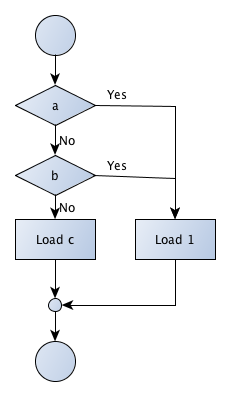
\includegraphics[scale=.5]{images/OrChain.png}
\end{center}
\caption{Program flow of an or chain}
\label{fig:orchain}
\end{figure}

%\lstset{language=[x86masm]Assembler, morekeywords={LV,TJMP,LIT}}

\begin{lstlisting}[float,caption={Assembler code of or-chain}, captionpos=b,label=cod:orchain]
...
lv 0, 32		# load value a
tjmp 8		# if true, jump to the end
lv 0, 36		# load value b
tjmp 8		# if true, jump to the end
lv 0, 40		# load value c
jmp 9			# result is determined by c only
lit 1
...
\end{lstlisting}
When generating this kind of code, we have to deal with the situation that the final addresses we have to jump to are not known in prior. Therefore, we have to construct a so-called or-chain, which work as follows. While parsing a conditional expression, we maintain an int variable holding the 

The translation of {\em and-}expressions works analogously.

%\section{Jumps in If- and While-Statements}

\chapter{Error Handling}
ErrorHandler.getInstance().raise(new ...));

\chapter{Attributed Grammar}
%\begin{atg}[4.5cm]
%\leongage &=& & \semantics{\begin{sem} \newline EmitOp(INC); \newline Emit2(0); \newline int inc\_addr = 1; \newline \end{sem}}\\
%&&Stat ";" \{Stat ";"\}. \\
%
%Stat & = & ident ":=" \atgsy{Expr}{\outattr op}  \alternative \\
%&& "PUT" \atgsy{Expr}{\outattr op}. \\
%
%\atgsy{Term}{\outattr op} &=& \atgsy{Fact}{\outattr op}  \\
%&& \{("*" &\semantics{\begin{sem} opcode = mul \end{sem}}\\
%&& \alternative "/" & \semantics{\begin{sem} opcode = div \end{sem}}\\
%&&) & \semantics{\begin{sem}EmitOp(\inattr opcode)\end{sem}}\\
%&&\atgsy{Fact}{\outattr op} & \semantics{\begin{sem}LoadVal(\inattr op)\end{sem}}
%\end{atg}

%\begin{atg}
%\completerule{NoBeard}{``unit'' identifier Block\in{identifier} ``;''}
%\leftside{Reference \out{op}}
%\rightside{identifier \out{name}}
%\sem{
%obj = findObject(name);
%op = obj.createOperand();
%}
%\where{op.getKind() == VARIABLE}
%\end{atg}

\bibliography{my_bibliography}{}
\bibliographystyle{alphaurl} % save alternatives are abbrvurl	alphaurl	plainurl	unsrturl

\end{document}  